\documentclass[12,twoside]{TFG-GM}
%\usepackage[active]{srcltx}
\usepackage{amsthm,amsmath,amssymb,amsfonts,amscd}
\usepackage{graphicx}
\usepackage{enumerate}
\usepackage[all]{xy}
\usepackage{booktabs}
%\usepackage[usenames]{xcolor}
%\usepackage{fancyhdr}
\usepackage{minted}
%%%%%Author packages if necessary
\usepackage{hyperref}
\usepackage[spanish]{babel}

\usepackage[utf8]{inputenc}
\usepackage[T1]{fontenc}
\usepackage{environ}

\usepackage{tikz}
%\usetikzlibrary{arrows}
\usetikzlibrary{positioning}
\usetikzlibrary{matrix}

\usepackage{pgfplots}
\pgfplotsset{compat=1.10}

\usepackage[nottoc]{tocbibind} %Adds "References" to the table of contents

\usepackage{neuralnetwork}
\usepackage{xcolor}
\usepackage{chronology}

%\usepackage[demo]{graphicx}
\usepackage{caption}
\usepackage{subcaption}
\usepackage{wrapfig}

% Theorem Environments: add extra ones at the end if you need it.

\newtheorem*{theoremA}{Theorem A}
\newtheorem{theorem}{Theorem}[section]

\newtheorem{proposition}[theorem]{Proposition}
\newtheorem{lemma}[theorem]{Lemma}
\newtheorem{corollary}[theorem]{Corollary}
\newtheorem{conjecture}[theorem]{Conjecture}

\theoremstyle{definition}
\newtheorem{definition}[theorem]{Definición}
\newtheorem{example}[theorem]{Example}

\theoremstyle{remark}
\newtheorem{remark}[theorem]{Remark}
\newtheorem*{remarknonumber}{Remark}
\newtheorem{observation}[theorem]{Observation}




%%%%%%%%%%%%%%%%%%
% macros/abbreviations: Include here your own.
%%%%%%%%%%%%%%%%%%

\newcommand{\N}{\ensuremath{\mathbb{N}}}

\DeclareCaptionType{equ}[][]
\DeclareCaptionLabelFormat{nospace}{#1 #2}
\captionsetup[equ]{name=Equación ,labelformat=nospace,labelsep=period}

%%%%%%%%%%%%%%%%%%
% tikz config
%%%%%%%%%%%%%%%%%%


\tikzset{basic/.style={draw,fill=blue!20,text width=1em,text badly centered}}
\tikzset{input/.style={basic,circle}}
\tikzset{weights/.style={basic,rectangle}}
\tikzset{functions/.style={basic,circle,fill=blue!10}}
\tikzstyle{arrow}=[draw, -latex]

\makeatletter
\newsavebox{\measure@tikzpicture}
\NewEnviron{scaletikzpicturetowidth}[1]{%
  \def\tikz@width{#1}%
  \def\tikzscale{1}\begin{lrbox}{\measure@tikzpicture}%
  \BODY
  \end{lrbox}%
  \pgfmathparse{#1/\wd\measure@tikzpicture}%
  \edef\tikzscale{\pgfmathresult}%
  \BODY
}
\makeatother

% Body of document

\titol{ Wordnet y Deep Learning: Una posible unión}
\titolcurt{Short title}
\authorStudent{Raquel Leandra Pérez Arnal}
\supervisors{(name of the supervisor/s of the master's thesis)}
\monthYear{Month, year}

%\msc[2010]{Primary  	55M25, 57P10, Secondary 55P15, 57R19, 57N15.}

\paraulesclau{keyword1, keyword2, keyword3, ...}
\agraiments{
Thanks to...}


\abstracteng{This should be an abstract in english, up to 1000 characters.}

%%%%%%%%%
\begin{document}
\pgfmathdeclarefunction{gauss}{2}{\pgfmathparse{1/(#2*sqrt(2*pi))*exp(-((x-#1)^2)/(2*#2^2))}%
}

\maketitle

\section{Conocimientos previos}
%\subsection{Machine Learning}
%%- Que es ml y por que está de moda. 
%%- Un poco de historia
%En los últimos años(fecha) ha estado en alza todo lo relacionado con \textit{Machine Learning}, pero, que es realmente machine learning? 
%Machine Learning es una aplicación de la Inteligencia Artificial que provee sistemas de la habilidad de mejorar a partir de una experiencia sin ser explícitamente programados para ello. 
%
%Su crecimiento se debe a: 
%\begin{itemize}
%\item Aumento de la capacidad computacional de los ordenadores. 
%\item Aumento de la cantidad de datos disponibles, junto la necesidad de analizarlos. 
%\end{itemize}
%
%En nuestro caso concreto nos centraremos en la aplicación de diversos métodos de ML a el problema de clasificación de imágenes. 


\subsection{Redes neuronales}
Una \textbf{red neuronal} es un modelo computacional inspirado en la forma de procesar información de las neuronas del cerebro. Las redes neuronales han generado una significativa cantidad de investigación e industria gracias a sus resultados en reconocimiento del habla, visión por computador y procesamiento de texto. Para dejar claro su funcionamiento explicaré primero el funcionamiento de una sola neurona, para después unirlo con la organización por capas de varias neuronas y finalmente explicar el algoritmo de \textit{backpropagation}. 

\subsubsection{Una neurona}

\begin{definition} 
La unidad de computación básica de una red neuronal es una \textbf{neurona}, también llamada nodo o unidad. Ésta, recibe una entrada sobre la que le aplica una función para generar na salida.
\end{definition}
Cada entrada (\textbf{x}) tiene asociado un peso (\textbf{w}), que es aprendido en base a su importancia relativa a otras entradas, a la salida y al objetivo de la red. La neurona  aplica una función (\textbf{f}) a la suma ponderada de las entradas como muestra la figura: 
%\begin{center}
%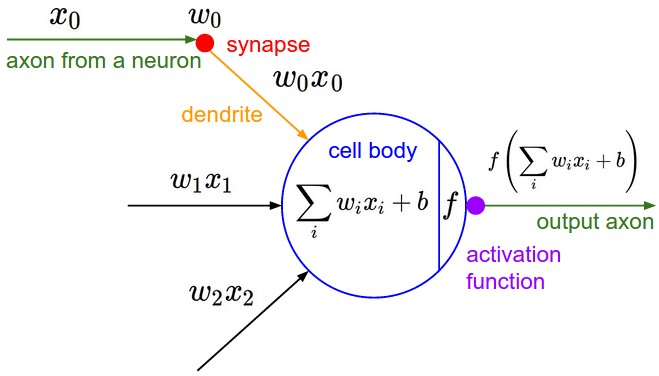
\includegraphics[width=0.5\textwidth]{Images/neuron_model.jpeg} 
%\end{center}

Además de los elementos ya comentados tendremos un término de sesgo (\textbf{b}), cuyo objetivo es proveer cada neurona con un valor entrenable que no dependa de la entrada. 

La salida de la neurona (\textbf{Y}) se calculara de la siguiente manera: 

$$
Y = f \left(\sum_i \omega_i x_i + b \right) 
$$

Llamaremos a \textbf{f} la \textbf{función de activación}, es una función (no lineal) diferenciable cuyo propósito es introducir no linealidad a la salida de la neurona. Ésto permite adaptar el modelo a problemas reales, puesto a que estos raramente son lineales. 

Las funciones de activación más utilizadas son: 

\begin{itemize}
\item Sigmoide: $f(x)=\frac{1}{1+e^{-x}}$
\begin{figure}[H]
\centering
%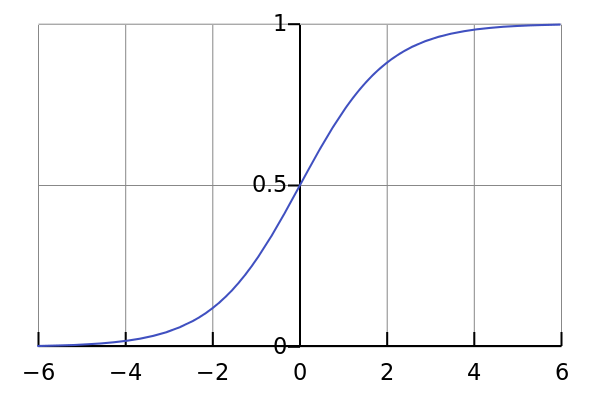
\includegraphics[width=0.5\textwidth]{Images/sigmoid.png} 
\begin{scaletikzpicturetowidth}{0.5\textwidth}
\begin{tikzpicture}[scale=\tikzscale]
    \begin{axis}[
        legend pos=north west,
        axis x line=middle,
        axis y line=middle,
        y tick label style={/pgf/number format/fixed,
                            /pgf/number format/fixed zerofill,
                            /pgf/number format/precision=1},
        grid = major,
        width=16cm,
        height=8cm,
        grid style={dashed, gray!30},
        xmin=-4,     % start the diagram at this x-coordinate
        xmax= 4,     % end   the diagram at this x-coordinate
        ymin= 0,     % start the diagram at this y-coordinate
        ymax= 1,     % end   the diagram at this y-coordinate
        %axis background/.style={fill=white},
        xlabel=$t$,
        ylabel=sig$(t)$,
        tick align=outside,
        enlargelimits=true]
      % plot the stirling-formulae
      \addplot[domain=-5:5, black, ultra thick,samples=500] {1/(1+exp(-1*x))};
      \addlegendentry{sig$(t)=\frac{1}{1+e^{-t}}$}
    \end{axis}
\end{tikzpicture}
\end{scaletikzpicturetowidth}
%\caption{Ejemplo de red neuronal}
\end{figure}
\item Tanh: $f(x)=\frac{2}{1+e^{-2x}}-1$
\begin{figure}[H]
\centering
%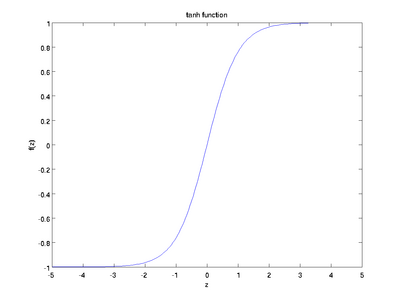
\includegraphics[width=0.5\textwidth]{Images/tanh.png} 
\begin{scaletikzpicturetowidth}{0.5\textwidth}
\begin{tikzpicture}[scale=\tikzscale]
    \begin{axis}[
        legend pos=north west,
        axis x line=middle,
        axis y line=middle,
        y tick label style={/pgf/number format/fixed,
                            /pgf/number format/fixed zerofill,
                            /pgf/number format/precision=1},
        grid = major,
        width=16cm,
        height=8cm,
        grid style={dashed, gray!30},
        xmin=-4,     % start the diagram at this x-coordinate
        xmax= 4,     % end   the diagram at this x-coordinate
        ymin= -1,     % start the diagram at this y-coordinate
        ymax= 1,     % end   the diagram at this y-coordinate
        %axis background/.style={fill=white},
        xlabel=$x$,
        ylabel=$tanh(x)$,
        tick align=outside,
        enlargelimits=true]
      % plot the stirling-formulae
      \addplot[domain=-5:5, black, ultra thick,samples=500] {2/(1+exp(-2*x)) - 1};
      \addlegendentry{$tanh(x)=\frac{2}{1+e^{-2x}}-1$}
    \end{axis}
\end{tikzpicture}
\end{scaletikzpicturetowidth}
\end{figure}

%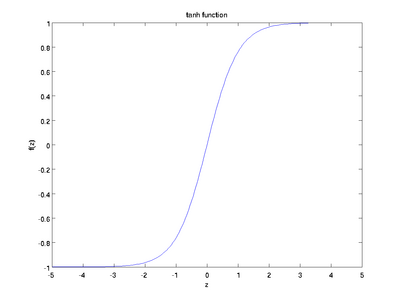
\includegraphics[scale=1]{Images/tanh.png} 
\item ReLU: $f(x)=max(0,x)$

\begin{figure}[H]
\centering
%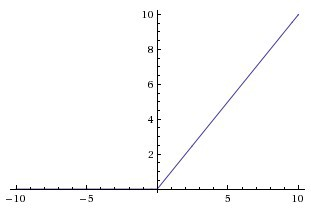
\includegraphics[width=0.5\textwidth]{Images/relu.jpeg} 
\begin{scaletikzpicturetowidth}{0.5\textwidth}
\begin{tikzpicture}[scale=\tikzscale]
    \begin{axis}[
        legend pos=north west,
        axis x line=middle,
        axis y line=middle,
        y tick label style={/pgf/number format/fixed,
                            /pgf/number format/fixed zerofill,
                            /pgf/number format/precision=1},
        grid = major,
        width=16cm,
        height=8cm,
        grid style={dashed, gray!30},
        xmin=-4,     % start the diagram at this x-coordinate
        xmax= 4,     % end   the diagram at this x-coordinate
        ymin= 0,     % start the diagram at this y-coordinate
        ymax= 4,     % end   the diagram at this y-coordinate
        %axis background/.style={fill=white},
        xlabel=$x$,
        ylabel=$relu(x)$,
        tick align=outside,
        enlargelimits=true]
      % plot the stirling-formulae
      \addplot[domain=-5:5, black, ultra thick,samples=500] {max(0,x)};
      \addlegendentry{$f(x)=max(0,x)$}
    \end{axis}
\end{tikzpicture}
\end{scaletikzpicturetowidth}
\end{figure}
%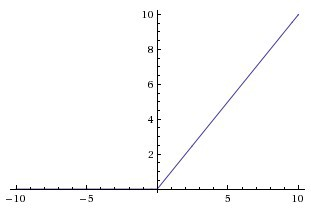
\includegraphics[scale=1]{Images/relu.png} 
\end{itemize}

%

Dotando una neurona de una función de pérdida en la salida podríamos convertirla en un clasificador lineal, pero la verdadera potencia del método viene dada al unir diversas neuronas en lo que llamaremos capas.
\begin{figure}[H]
\centering
 \begin{tikzpicture}
        \node[functions] (center) {$f$};
        \node[below of=center,font=\scriptsize,text width=4em] {Función de activación};

        \node[right of=center] (right) {};
            \path[draw,arrow] (center) -- (right);
        \node[functions,left=3em of center,text width=3em ] (left) {$\sum w_i x_i$};
            \path[draw,arrow] (left) -- (center);
        \node[weights,left=3em of left] (2) {$w_2$} -- (2) node[input,left of=2] (l2) {$x_2$};
            \path[draw,arrow] (l2) -- (2);
            \path[draw,arrow] (2) -- (left);
        \node[below of=2] (dots) {$\vdots$} -- (dots) node[left of=dots] (ldots) {$\vdots$};
        \node[weights,below of=dots] (n) {$w_n$} -- (n) node[input,left of=n] (ln) {$x_n$};
            \path[draw,arrow] (ln) -- (n);
            \path[draw,arrow] (n) -- (left);
        \node[weights,above of=2] (1) {$w_1$} -- (1) node[input,left of=1] (l1) {$x_1$};
            \path[draw,arrow] (l1) -- (1);
            \path[draw,arrow] (1) -- (left);
        \node[weights,above of=1] (0) {$w_0$} -- (0) node[input,left of=0] (l0) {$1$};
            \path[draw,arrow] (l0) -- (0);
            \path[draw,arrow] (0) -- (left);
        \node[below of=ln,font=\scriptsize] {Pesos};
        \node[below of=n,font=\scriptsize] { Entrada};
    \end{tikzpicture}
    \caption{Ejemplo de una neurona \label{fig:perceptron}}
\end{figure}

\subsubsection{Organización por capas}
Las redes neuronales se modelizan como una colección de neuronas conectadas en un grafo acíclico, comúnmente organizado por capas. El tipo más común de capa es la capa completa(\textit{fully-connected layer}), en el que todas las neuronas de una capa están conectadas con las de la capa posterior a ésta, mientras que no comparten ninguna conexión con las de su propia capa, como muestra la figura \ref{fig:red neuronal}. %Si tenemos diversas capas ocultas diremos que se trata de una red profunda (\textit{deep network}).
\begin{figure}
\begin{center}
\begin{neuralnetwork}[height=4]
		\newcommand{\nodetextclear}[2]{}
		\newcommand{\nodetextx}[2]{$x_#2$}
		\newcommand{\nodetexty}[2]{$y_#2$}
		\inputlayer[count=4, bias=false, title=Capa \\de entrada, text=\nodetextx]
		\hiddenlayer[count=5, bias=false, title=Capa \\ oculta 1, text=\nodetextclear] \linklayers
		\hiddenlayer[count=5, bias=false, title=Capa \\ oculta 2, text=\nodetextclear] \linklayers
		\outputlayer[count=3, title=Capa\\ de salida, text=\nodetexty] \linklayers
	
	\end{neuralnetwork}
	
\end{center}
\caption{Ejemplo de red neuronal \label{fig:red neuronal}}
\end{figure}
La red neuronal más básica la podemos dividir en: 
\begin{enumerate}
\item Neuronas de entrada: Proveen la red de información del exterior, consisten en los datos de entrada, todo su conjunto se conoce como la capa de entrada. 
\item Neuronas ocultas: Las neuronas ocultas no tienen conexión directa con el exterior. Solo calculan y transfieren información de la entrada a la salida. La colección de las neuronas ocultas se denomina las capas ocultas.
\item Neuronas de salida: Colectivamente denominados capa de salida y son responsables de generar la salia de la red neuronal calculada a partir de la entrada y procesada por varias capas. 
\end{enumerate}

%Dos ejemplos de redes de este tipo serían el perceptron y el multilayer perceptron. 
Por tanto nos queda una estructura formada por pesos ordenados en distintos tipos de capas. Cada peso de la red es un parámetros que necesitamos que la red aprenda, y de esta forma corresponda con el resultado esperado (permitiendo un cierto error). Para ello utilizaremos el algoritmo de \textit{backpropagation}, que explicaremos en el siguiente apartado \ref{sec:backpropagation}.

\subsubsection{Entrenar la red: Backpropagation}\label{sec:backpropagation}
Finalmente, queda explicar como entrenar los distintos parámetros para que se adapten a los datos, para ello se utiliza \textbf{backpropagation}.

El algoritmo de backpropagation empieza con un \textit{fordward pass}(una evaluación en la que se procesa la entrada desde el principio hasta generar la salida de acuerdo con el estado actual de la red) por toda la red, la predicción dada por la red se compara con la salida esperada 
y se calcula un error utilizando la función de pérdida (por ejemplo la de mínimos cuadrados). La pérdida calculada se utiliza para actualizar los pesos de la última capa, buscando los valores de éstos que la minimizan.

\textbf{TODO: Añadir un ejemplo, explicar bien backprop}

La complejidad reside en optimizar los pesos de las capas que no están conectadas directamente con la salida. Para resolver esto backpropagation utiliza la regla de la cadena, que permite calcular derivadas de capas previas, y de esta forma actualizar los pesos de las capas restantes. 

Tradicionalmente, el cambio de pesos se ha computado usando el algoritmo de optimización llamado \textit{ Stochastic Gradient Descent}, un método iterativo de minimización.

De esta forma, aplicando backpropagation iterativamente podemos estimar los pesos de todas las capas de una red neuronal para un problema dado.




\newpage

\subsection{Redes convolucionales}
%- Explicar el problema inicial (clasificación de imágenes) y por que es difícil.
%- Explicar que es una red convolucional 
\begin{definition}
Una \textbf{red convolucional} es una secuencia de capas de diferentes tipos, donde,  al menos una de las capas es una capa convolucional. 
\end{definition}
Las redes convolucionales son muy similares a las redes neuronales explicadas, las mayores diferencias son que contienen un tipo especial de neuronas (las neuronas convolucionales) y que asume explícitamente que la entrada son datos con una estructura concreta(como por ejemplo imágenes), lo que permite añadir ciertas propiedades a la arquitectura. Esto permite hacer un \textit{fordward pass} más eficiente de implementar y reducir significativamente la cantidad de parámetros.

Una neurona convolucional es aquella que opera con una convolución\cite{wikiconv}.

\begin{definition} \label{def:convolution}
Una \textbf{convolución} es una aplicación matemática cuya entrada son dos funciones de valores reales (\textbf{x} y \textbf{w}) y cuya salida es otra función (\textbf{s}). 

Usualmente se denota como $s(t) = (x * w)(t) $.

En el contexto de redes convolucionales llamaremos a \textit{x} \textit{entrada}, a \textit{w} kernel y a la salida \textit{s} \textit{feature map}.
\end{definition}

Nótese que la definición no depende de la dimensión del espacio, es decir, que podemos definir una convolución para tantas dimensiones como necesitemos.
En el caso concreto de una imagen \textit{I} (de dos dimensiones) y un kernel \textit{K}, la convolución quedaría como: 
\begin{equ}[H]
\begin{equation}
S(i,j) = (I * K)(i,j) = \sum_m \sum_n I(i +m, j+n) K(m,n)
\end{equation}
\caption{Convolución}
\end{equ}


%\begin{center}
%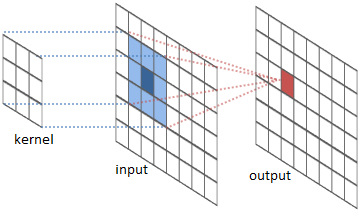
\includegraphics[width = 0.5\textwidth]{Images/convolution2.png} 
%\end{center}
\begin{definition}
Una \textbf{función de kernel}
\end{definition}
 

Típicamente las neuronas convolucionales tienen una entrada limitada, es decir están conectadas solo a un subconjunto de las neuronas de la capa anterior, de esta forma cada neurona se centra solo en parte de la entrada, lo que significa el aprendizaje de las neuronas individuales cuando hay entradas de muchas dimensiones. En contraste, las neuronas de una capa completa están conectadas a todas las neuronas de la capa anterior. %En este caso detallaremos el caso de datos en dos dimensiones, por ser el caso más común y por ser más fácil de entender. Una vez comprendida una convolución 2-dimensional, el lector puede extrapolar a tantas dimensiones como sea necesario.
De esta forma se reducen la cantidad de parámetros de la red.
%Para definir su conectividad de entrada, las neuronas convolucionales asumen la existencia de una cierta estructura en los datos. 
%Para capturar patrones consistentes, las neuronas convolucionales están conectadas a un conjunto de neuronas de la capa anterior que definen parcelas cuadradas (en el caso de convoluciones de dos dimensiones).



Por su conectividad limitada, las capas convolucionales pueden centrarse en una parcela particular de la entrada. El conjunto de pesos (que sería equivalente al kernel comentado en la definición \ref{def:convolution}) aprendido por esta parcela puede ser relevante para las otras parcelas de la entrada, por tanto, podemos definir neuronas similares que utilicen el mismo kernel, pero que se enfoquen en otra parte de la entrada. Esta idea se conoce como "weight sharing",por que varias neuronas de la misma capa están definidas por un conjunto común de pesos, esto permite tener una considerable cantidad de neuronas utilizando los mismos parámetros. Esto puede ayudar a detectar los mismos patrones en diferentes partes de la entrada. Por ejemplo si tenemos una neurona que detecta ojos, al pasarla por una foto con una cara se activará dos veces.  


\begin{figure}[H]

\begin{center}
%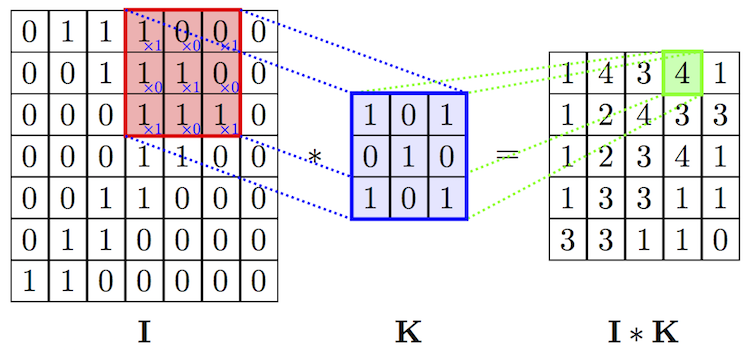
\includegraphics[width = 0.5\textwidth]{Images/convolve.png} 
\begin{tikzpicture}

	\matrix (mtr) [matrix of nodes,row sep=-\pgflinewidth, nodes={draw}]
	{
		0 & 1 & 1 & |[fill=red!30]| 1 & |[fill=red!30]| 0 & |[fill=red!30]| 0 & 0\\
		0 & 0 & 1 & |[fill=red!30]| 1 & |[fill=red!30]| 1 & |[fill=red!30]| 0 & 0\\
		0 & 0 & 0 & |[fill=red!30]| 1 & |[fill=red!30]| 1 & |[fill=red!30]| 1 & 0\\
		0 & 0 & 0 & 1 & 1 & 0 & 0\\
		0 & 0 & 1 & 1 & 0 & 0 & 0\\
		0 & 1 & 1 & 0 & 0 & 0 & 0\\
		1 & 1 & 0 & 0 & 0 & 0 & 0\\
	};

	\draw[very thick, red] (mtr-1-4.north west) rectangle (mtr-3-6.south east);

	\node [below= of mtr-5-4.south] (lm) {$\bf I$};

	\node[right = 0.2em of mtr] (str) {$*$};

	\matrix (K) [right=0.2em of str,matrix of nodes,row sep=-\pgflinewidth, nodes={draw, fill=blue!30}]
	{
		1 & 0 & 1 \\
		0 & 1 & 0 \\
		1 & 0 & 1 \\
	};
	\node [below = of K-3-2.south] (lk) {$\bf K$};

	\node [right = 0.2em of K] (eq) {$=$};

	\matrix (ret) [right=0.2em of eq,matrix of nodes,row sep=-\pgflinewidth, nodes={draw}]
	{
		1 & 4 & 3 & |[fill=green!30]| 4 & 1\\
		1 & 2 & 4 & 3 & 3\\
		1 & 2 & 3 & 4 & 1\\
		1 & 3 & 3 & 1 & 1\\
		3 & 3 & 1 & 1 & 0\\
	};
	\node [below = of ret-4-3.south] (lim) {${\bf I} * {\bf K}$};

	\draw[very thick, green] (ret-1-4.north west) rectangle (ret-1-4.south east);

	\draw[densely dotted, blue, thick] (mtr-1-4.north west) -- (K-1-1.north west);
	\draw[densely dotted, blue, thick] (mtr-3-4.south west) -- (K-3-1.south west);
	\draw[densely dotted, blue, thick] (mtr-1-6.north east) -- (K-1-3.north east);
	\draw[densely dotted, blue, thick] (mtr-3-6.south east) -- (K-3-3.south east);

	\draw[densely dotted, green, thick] (ret-1-4.north west) -- (K-1-1.north west);
	\draw[densely dotted, green, thick] (ret-1-4.south west) -- (K-3-1.south west);
	\draw[densely dotted, green, thick] (ret-1-4.north east) -- (K-1-3.north east);
	\draw[densely dotted, green, thick] (ret-1-4.south east) -- (K-3-3.south east);

	\matrix (K) [right=0.2em of str,matrix of nodes,row sep=-\pgflinewidth, nodes={draw, fill=blue!10}]
	{
		1 & 0 & 1 \\
		0 & 1 & 0 \\
		1 & 0 & 1 \\
	};

	\draw[very thick, blue] (K-1-1.north west) rectangle (K-3-3.south east);

	\node[anchor=south east, inner sep=0.01em, blue] at (mtr-1-4.south east) (xx) {\scalebox{.5}{$\times 1$}};
	\node[anchor=south east, inner sep=0.01em, blue] at (mtr-1-5.south east) (xx) {\scalebox{.5}{$\times 0$}};
	\node[anchor=south east, inner sep=0.01em, blue] at (mtr-1-6.south east) (xx) {\scalebox{.5}{$\times 1$}};
	\node[anchor=south east, inner sep=0.01em, blue] at (mtr-2-4.south east) (xx) {\scalebox{.5}{$\times 0$}};
	\node[anchor=south east, inner sep=0.01em, blue] at (mtr-2-5.south east) (xx) {\scalebox{.5}{$\times 1$}};
	\node[anchor=south east, inner sep=0.01em, blue] at (mtr-2-6.south east) (xx) {\scalebox{.5}{$\times 0$}};
	\node[anchor=south east, inner sep=0.01em, blue] at (mtr-3-4.south east) (xx) {\scalebox{.5}{$\times 1$}};
	\node[anchor=south east, inner sep=0.01em, blue] at (mtr-3-5.south east) (xx) {\scalebox{.5}{$\times 0$}};
	\node[anchor=south east, inner sep=0.01em, blue] at (mtr-3-6.south east) (xx) {\scalebox{.5}{$\times 1$}};

\end{tikzpicture}

\end{center}
\caption{Ejemplo de la forma de operar una convolución sobre una imagen.
\label{fig:conv}
}

\end{figure}

En la figura \ref{fig:conv} podemos ver un ejemplo del funcionamiento de una convolución con un kernel de tamaño 9 sobre una imagen, en el ejemplo podemos observar como se comparten los pesos a la hora de calcular el resultado.


Finalmente queda comentar los tipos de capa más comunes en una red convolucional: 
\begin{itemize}
\item Capa convolucional, capas formadas por neuronas convolucionales, la mayoría de capas de una red convolucional serán de este tipo.
\item Capa completa, es una capa donde todas las neuronas están conectadas entre ellas. Se suele utilizar como capa de clasificación. 
\item \textit{Pooling Layer}, consiste en una capa que aplica una reducción matemática a su input(como una media o un max). El objetivo es aportar un cierto grado de invariancia espacial (imágenes equivalentes en diferentes posiciones), además reducen el tamaño de la salida de la capa, lo que provoca una reducción de la complejidad de la red.
\end{itemize}

\begin{center}
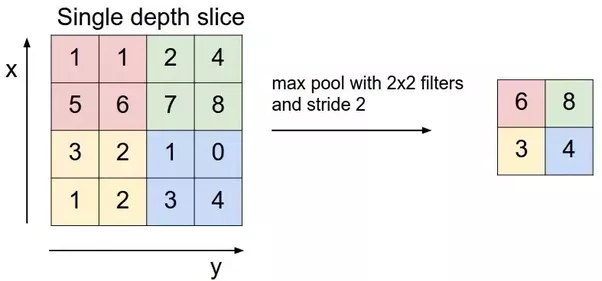
\includegraphics[width = 0.5\textwidth]{Images/pooling1.png} 
\end{center}

Otro concepto que utilizaremos a lo largo del documento es el de \textit{feature}.

\begin{definition}
Llamaremos \textbf{feature} a los distintos subconjuntos de neuronas que ayudan a una red a cumplir con la tarea para la que fue diseñada, se generan al entrenar los pesos y pueden tener distintos grados de abstracción. 
\end{definition}

En redes convolucionales, la disposición por capas permite representar la información más compleja a partir de otra más simples. Por tanto puede acabar extrayendo \textit{features} abstractas en la figura \ref{fig:deepconcept}, podemos ver un ejemplo de \textit{features} de distinto nivel de abstracción. Por ejemplo, si queremos clasificar diferentes animales, la presencia de \textit{pico} sería una \textit{feature}. 


\begin{figure}[h]
\centering
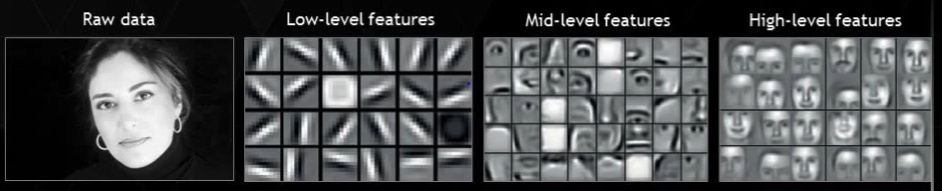
\includegraphics[width = 0.8\textwidth]{Images/deepConcept.png} 
\caption{Ejemplo de features \label{fig:deepconcept}}
\end{figure}

\newpage
\subsection{Transfer Learning}
%- Explicar que es transfer learning 

En la práctica pocas personas entrenan una red profunda desde cero (con inicialización aleatoria), puesto a que éstas tienen unos requisitos bastante exigentes a la hora de ser entrenadas. 

Los mayores problemas que puedes encontrar son: 
\begin{enumerate}
\item A causa de la gran cantidad de parámetros a entrenar que tiene una red profunda necesitas un \textbf{conjunto de datos de gran tamaño}.
\item El \textbf{coste computacional} de entrenar la red, determinado por el número de parámetros. 
\item La búsqueda de \textbf{hiper-parámetros} (valores de los que depende el modelo) óptimos. 

La forma de obtener los hiper-parámetros es, entrenar la red para cada uno de los hiper-parámetros que hayamos considerado y, utilizando una partición de validación (o el método de \textit{cross-validation}) comparar los distintos resultados.  

Ésto incrementa los problemas \textit{1}, al necesitar una partición de validación necesitaremos más datos, y \textit{2}, el coste computacional se multiplica por cada vez que haya que entrenar la red, que puede ser varias veces por cada hiper-parámetro que tengamos.
\end{enumerate}
Por tanto, es común pre-entrenar una red convolucional en un conjunto de datos significativamente grande y usar la red convolucional como inicialización o como extractor fijo de características de la tarea de interés. 
\begin{definition}
Llamaremos \textbf{transfer learning} al campo de estudio que reutiliza el lenguaje de representación de un problema(que llamaremos problema origen o \textit{Source}) para resolver otro(que llamaremos objetivo o \textit{Target}). 

A la hora de utilizar \textbf{transfer learning} tenemos dos componentes base:  Un dominio $\mathcal{D}$ definido por un conjunto de instancias de datos con una distribución de probabilidades y una tarea $\mathcal{T}$, definida a partir de un conjunto de clases y una función objetivo.

Para un problema de \textit{transfer learning} usaremos la notación: 
\begin{itemize}
\item Problema origen: $(\mathcal{T_S},\mathcal{D_S})$
\item Problema objetivo: $(\mathcal{T_T},\mathcal{D_T})$
\end{itemize}

\end{definition}

Los dos casos más comunes de transfer learning son: 

\begin{itemize}
\item \textbf{Fine-tuning} La primera estrategia consiste en inicializar los datos desde un estado no aleatorio (tomando los pesos ya entrenados), y a continuación, entrenar la red sobre estos datos. 
De esta manera puedes reducir significativamente el conjunto de datos necesario para entrenarla, sin embargo, sigue necesitando tiempo para optimizar los múltiples hiper-parámetros involucrados en el proceso y una cantidad significativa de recursos computacionales. 
%En el caso de redes convolucionales esto se debe a que las primeras capas tienden a ser bastante generales.


\item \textbf{Feature Extraction} Consiste en procesar un conjunto de datos a través de una red neuronal ya entrenada y extraer valores de activación para que puedan ser utilizados por otro mecanismo de aprendizaje. Este método es aplicable a conjuntos de datos de cualquier tamaño, puesto a que cada dato es procesado independientemente. Además tiene un menor coste computacional, ya que no tiene que entrenar la red y no requiere la optimización de hiper-parámetros. Por estos motivos las aplicaciones de \textit{transfer learning for feature extraction} están limitadas solo a las  capacidades de los métodos que utilices encima de la representación profunda obtenida. 


\end{itemize}

En nuestro caso nos centraremos en \textit{transfer learning for features extraction} \cite{behaviourcnn}. 




\newpage

\section{Trabajo Relacionado}

\subsection{Full-Network embedding}

En general en \textit{transfer learning for feature extraction} es común tomar los valores de activación de una sola capa cercana a la salida, como podemos ver en la figura \ref{fig:base}. El resto de capas se descartan por 
"ser poco probable que contengan una representación mejor", sin embargo es conocido que todas las capas de una red profunda pueden contribuir a caracterizar los datos de diferentes maneras. Esto implica que la representación más versátil y rica que puede ser generada por un proceso de \textit{features extraction} debe incluir todas las capas de la red,es decir, debe definir un \textit{full-network embedding}. 
\begin{figure}[H]
\centering
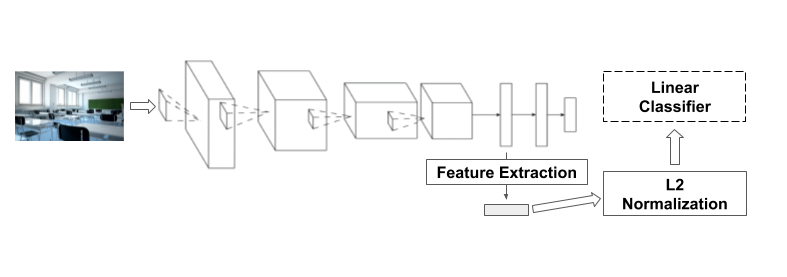
\includegraphics[width = 0.8\textwidth]{Images/basecrop.png} 
\caption{Estructura básica que se suele utilizar en \textit{feature extraction}
\label{fig:base}}
\end{figure}
Dado un conjunto de datos \textit{t1}, queremos representarlo en el lenguaje aprendido para una tarea \textit{t0}. Para ello el \textit{full-network embedding} se divide en 4 pasos: 
\begin{itemize}
\item El primer paso es hacer un \textbf{forward pass} de cada instancia de datos de \textit{t1} a través del modelo entrenado en \textit{t0}, guardando todos los valores de activación de cada capa de la red, (tanto las convolucionales como las completas). 

\item El segundo paso consiste en un \textbf{spatial average pooling} en los filtros convolucionales. Como se ha explicado en el capítulo sobre redes convolucionales, un filtro convolucional genera varias activaciones para una entrada, para darle la capacidad de obtener información espacial.  El objetivo de este paso es obtener un solo valor de activación para cada filtro, evitando así un aumento de la dimensionalidad. Los valores resultantes se concatenan a los de las capas completas en un solo vector, para generar el \textit{embedding} completo.

\item El tercer paso es una \textbf{estandarización de características}. Puesto a que los valores del \textit{embedding} provienen de distintos tipos de neuronas en distintos puntos de la red hace falta una estandarización. El valor estandarizado de cada categoría se obtiene calculando la media y la desviación típica del conjunto de datos de entrenamiento. De esta forma se pueden integrar los distintos valores en el \textit{embedding}. 

\begin{figure}

\centering
\begin{tikzpicture}

\begin{axis}[no markers, domain=0:10, samples=100,
axis lines*=left, xlabel=, ylabel=,
height=6cm, width=10cm,
xticklabels={ , , -1 , $ft^-$ , 0 , $ft^+$ , 1},
ytick=\empty,
enlargelimits=false, clip=false, axis on top,
grid = major]
\addplot [fill=cyan!20, draw=none, domain=-1:1] {gauss(0,1)} \closedcycle;
\addplot [fill=blue!20, draw=none, domain=-3:-1] {gauss(0,1)} \closedcycle;
\addplot [fill=blue!20, draw=none, domain=1:3] {gauss(0,1)} \closedcycle;
\end{axis}
\end{tikzpicture}
\caption{
\label{fig:caracterization}}
\end{figure}

\item Finalmente se aplica una \textbf{discretización de características} para evitar problemas al intentar explorar un espacio de dimensión tan grande. Ésta discretización consiste en tomar unos límites que dependen de los datos, $ft^-$ y $ft^+$ y reemplazar los valores que tienen un valor atípicamente bajo (todos los valores $x < ft^-$) por un -1, los que tienen un valor típico (todos los valores $ ft^- < x < ft^+$) por un 0 y los que tienen un valor atípicamente alto (todos los valores $ ft^+ < x$) por un 1, como podemos ver en la representación gráfica \ref{fig:caracterization}. Para encontrar los límites se basan en \cite{behaviourcnn}, donde dan una visión estadística sobre como evaluar la importancia de las diferentes características de una red convolucional comparando las activaciones para una clase concreta respecto al resto de clases del conjunto de datos. De esta forma los autores de \cite{behaviourcnn} separan las características en tres conjuntos: \textit{característico por presencia}, \textit{no característico} y \textit{característico por ausencia}.

\end{itemize}
\begin{figure}[h]
\label{fig:fne}
\centering
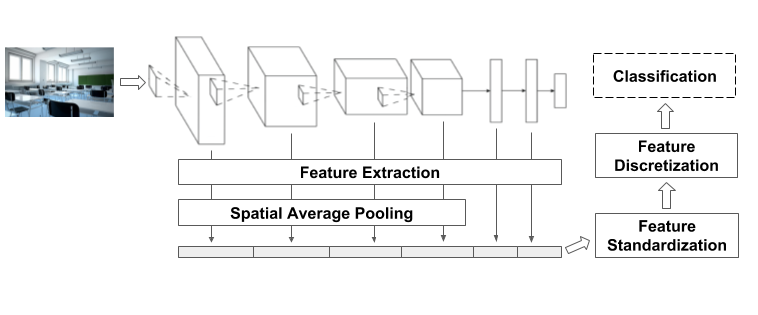
\includegraphics[width = 0.8\textwidth]{Images/cropfne.png} 
\caption{Estructura del \textit{full-network embedding}}
\end{figure}




\subsection{Wordnet}

\textbf{Wordnet} es una base de datos que contiene nombres, verbos, adjetivos y adverbios en conjuntos de sinónimos (que llamaremos \textit{synsets}). Los synsets están conectados entre ellos por medio de relaciones conceptuales, semánticas y léxicas. Utilizando los \textit{synsets} y sus relaciones, se puede generar un grafo que puede ser utilizado para distintos objetivos, como lingüística computacional y procesamiento del lenguaje natural. 

En concreto utilizaremos las relaciones de: 
\begin{itemize}

\item \textbf{Sinonimia} : dos palabras son sinónimos si tienen el mismo significado (ej, gato y minino).
\item \textbf{Hiponimia}: una palabra es hipónimo de otra si su significado es más específico que el de ésta (ej, silla es hipónimo de mueble). 
\item \textbf{Hipernimia}: una palabra es hiperónimo de otra si su significado es menos específico que el de ésta (ej, perro es hiperónimo de dálmata). 
 
\end{itemize}

\begin{figure}[H]
\centering

\begin{tikzpicture}[sibling distance=10em,
  every node/.style = {shape=rectangle, rounded corners,
    draw, align=center,
    top color=blue!20, bottom color=blue!20},
    edge from parent/.style={draw,-latex}
    ]
  \node {Ser Vivo}
  	child{ node {Mamífero}
    	child{ node {Perro}}
    	child{node {Gato}}
    };
\end{tikzpicture}
\caption{Ejemplo de hipónimos}
\end{figure}

\subsection{Imagenet}

\textbf{Imagenet} es una base de datos de imágenes organizada utilizando la jerarquía de \textit{wordnet}. Su principal objetivo es dotar a los investigadores en campos relacionados con visión artificial de una base de datos a gran escala con la que poder trabajar. Actualmente consta de 14,197,122 imágenes y  21841 \textit{synsets} indexados.  

Para el full-network embedding utilizaron el subconjunto correspondiente al reto de \textit{imagenet} de 2012 de reconocimiento de imágenes. 

Éste consta de:
\begin{itemize}
\item Un conjunto de datos de entrenamiento de 1.2 millones de muestras y 1000 categorías diferentes.
\item Un conjunto de datos de validación de 50000 muestras y 1000 categorías. 
\end{itemize}

Entre las posibles categorías podemos encontrar \textit{synsets} de diferentes niveles de especificación, por ejemplo tenemos las categorías: perro, dálmata, pastor alemán... 
\newpage
\section{Enfoque}

En nuestro caso estudiaremos un \textit{full-network embedding} obtenido a partir de la tarea origen  $(\mathcal{T_S} = $Clasificación de imágenes$,\mathcal{D_S} =$ 1.2 M imágenes de imagenet con sus correspondientes clases$ )$ y una tarea de destino $(\mathcal{T_T} = $Clasificación de imágenes$,\mathcal{D_T} =$ 50000 imágenes de imagenet con sus correspondientes clases$ )$. Es decir, partiendo de una red convolucional entrenada con todo el conjunto de datos de entrenamiento de imagenet, hemos generado un lenguaje de representación para el conjunto de datos de validación de imagenet. Lo que resulta en el \textit{full-network embedding} con el que trabajaremos. 

El \textit{full-network embedding} consiste en una matriz de tamaño 50000 muestras por 12416 características, cuyos valores están en $\{-1,0,1\}$. Para cada muestra también tenemos su correspondiente clasificación(un valor entre 0 y 999 que representa la clase de imagenet con la que fue clasificado).

Es importante remarcar el significado de las diferentes categorías.
\begin{itemize}
\item Si el valor para una imagen concreta es 1 significa que esta es representativa por presencia. Es decir, que dentro del contexto del conjunto de datos \textit{Target}, es una \textit{feature} característica de una clase concreta.
\item Si el valor para una imagen concreta es 0 significa que esa característica no es representativa.
\item Si el valor para una imagen concreta es -1 significa que es representativa por ausencia. 
\end{itemize}

Hemos de tener en cuenta que estas definiciones son con respecto a $\mathcal{D_T}$, es decir, respecto al nuevo espacio de representación. 

Por ejemplo si tenemos como datos objetivo un conjunto de coches tendremos que las features que se activen con las ruedas no serán representativas, puesto a que todos los coches tienen, las categorías que se activen con el techo de un coche serán representativas por ausencia para clasificar descapotables mientras que las que se activen para la capota serán representativas por presencia. 

Las características están ordenadas en capas de la siguiente manera: 
\begin{figure}[H]
\label{}
\centering
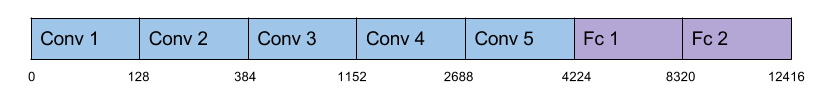
\includegraphics[width = 0.8\textwidth]{Images/croplayer.png} 
\caption{La disposición de las características por capas}
\end{figure}
%'fc6': [4224, 8320],  # 14
%			'fc7': [8320, 12416],  # 15
%			'conv1': [0, 128],  # 16
%			'conv2': [128, 384],  # 17
%			'conv3': [384, 1152],  # 18
%			'conv4': [1152, 2688],  # 19
%			'conv5': [2688, 4224],  # 20

%Además tomamos 3 embeddings diferentes:
%\begin{itemize}
%\item El básico con los límites en $ft^- = -0.25$ y $ft^+ = +0.25$ 
%\item Un embedding más restrictivo con los límites en $ft^- = -0.19$ y $ft^+ = +0.19$ 
%\item Un embedding menos restrictivo con los límites en $ft^+ = -0.31$ y $ft^+ = +0.31$ 
%\end{itemize}

Y finalmente, de todos los \textit{synsets} posibles tomamos dos conjuntos diferentes: 

\begin{figure}[H]
\centering
\begin{subfigure}{.5\textwidth}
  \centering
  %\includegraphics[width=.4\linewidth]{image1}
\begin{tikzpicture}[sibling distance=10em,
  every node/.style = {shape=rectangle, rounded corners,
    draw, align=center,
    top color=cyan!20, bottom color=cyan!20},
    edge from parent/.style={draw,-latex}
    ]
  \node {Ser Vivo}
  	child{ node {Mamífero}
    	child{ node {Perro}
			child{node {Perro de caza}    	
    		}
    	}
    };
\end{tikzpicture}
  \caption{Seres vivos}
  \label{fig:sub1}
\end{subfigure}%
\begin{subfigure}{.5\textwidth}
  \centering
  \begin{tikzpicture}[sibling distance=10em,
  every node/.style = {shape=rectangle, rounded corners,
    draw, align=center,
    top color=red!20, bottom color=red!20},
    edge from parent/.style={draw,-latex}
    ]
  \node {Artefacto}
  	child{ node {Instrumento}
    	child{ node {Transporte}
			child{node {Vehículo}    	
    		}
    	}
    };
\end{tikzpicture}
  \caption{Objetos}
  \label{fig:sub2}
\end{subfigure}
\caption{Conjuntos de synsets que estudiaremos \label{fig:synsets}}

\end{figure}

Hemos tomado estos dos conjuntos por estar distribuidos de una forma bastante uniforme entre las clases, como veremos en el capítulo \ref{se:stats}, y por ser de dos ''ramas'' lo más diferentes posibles, para poder comparar el comportamiento del embedding en ambos casos. 

 
\subsection{Objetivos}
Partiendo de los datos comentados y del trabajo publicado en \cite{fne} tomamos varios \textbf{objetivos} a partir de los que desarrollar el trabajo.

\begin{itemize}
\item Analizar el \textit{embedding} dado y elcomportamiento de las \textit{features} en las distintas capas. 
\item Analizar si hay alguna relación entre los embeddings de las diferentes clases y synsets relacionados con ellas (sus hipónimos e hipérnimos). 
\end{itemize}

\subsection{Estadísticas}\label{se:stats}
La finalidad de este capítulo es hacer un estudio inicial de los datos de los que se dispone, es decir, de los correspondientes a los distintos \textit{embeddings} y a los \textit{synsets} que hemos tomado para el estudio. 

\subsubsection{Embedding}
Primero de todo estudiaremos las estadísticas generales del \textit{embeddings}. 

Para empezar comparamos la cantidad de elementos de cada \textit{feature} en los distintos \textit{embeddings}. 

\begin{figure}[ht] 
	\centering
	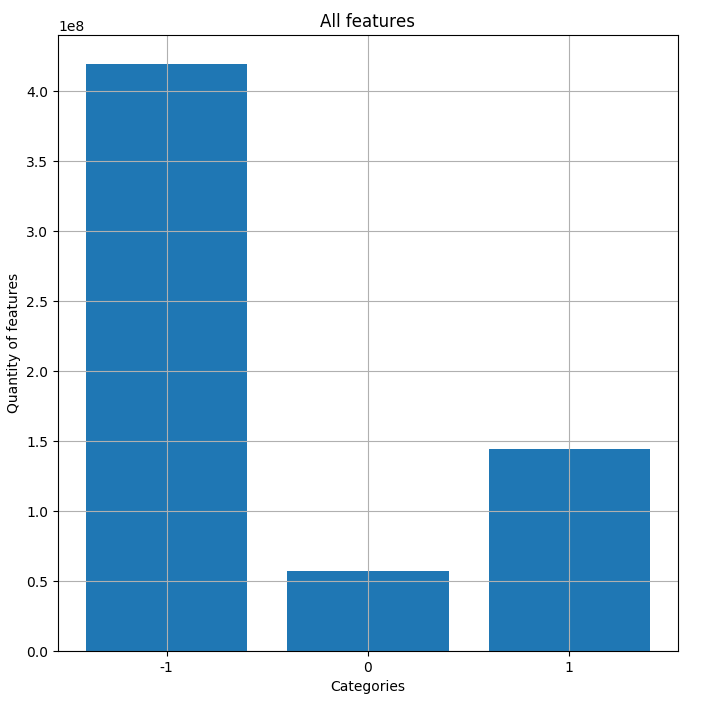
\includegraphics[width=0.4\textwidth] {Images/plots/25/quantity_of_features_bar.png}
	\caption{ 
	\label{fig:totalfeatures}}


\end{figure}

En la figura \ref{fig:totalfeatures} podemos observar que la cantidad total de -1 es significativamente mayor. Teniendo en cuenta que al hacer \textit{transfer learning} se suele pasar de un conjunto de datos más general a uno más específico que haya más \textit{features} características por ausencia es coherente. Más adelante veremos también como se distribuyen las categorías entre las diferentes capas del \textit{embedding}. 


Observamos también como se distribuyen las \textit{features} respecto al conjunto de imágenes que tenemos. 

\begin{figure}[ht] 
	\centering
	\begin{subfigure}[b]{0.3\textwidth}
		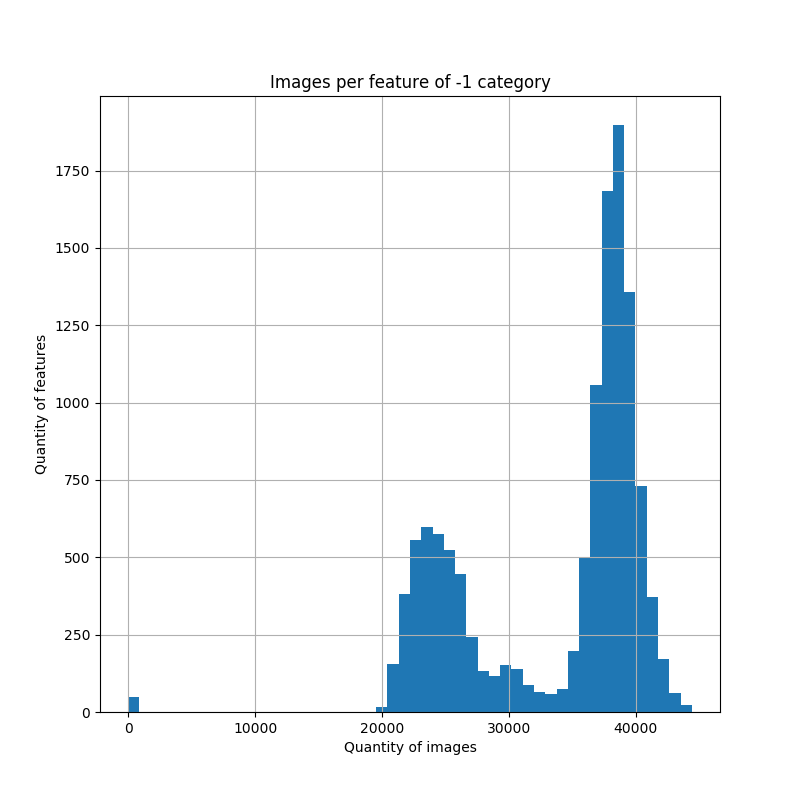
\includegraphics[width=\textwidth] {Images/plots/25/Images_per_feature_of_-1_category.png}
		\caption{Categoría -1}
	\end{subfigure}
	\begin{subfigure}[b]{0.3\textwidth}
		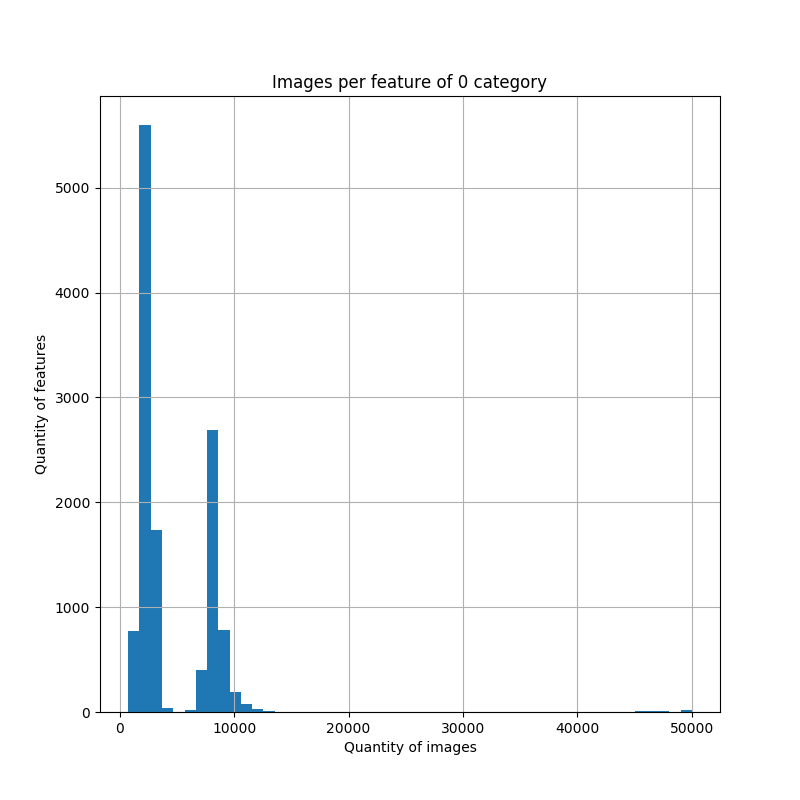
\includegraphics[width=\textwidth]  {Images/plots/25/Images_per_feature_of_0_category.png}
		\caption{Categoría 0}
	\end{subfigure}
	\begin{subfigure}[b]{0.3\textwidth}
		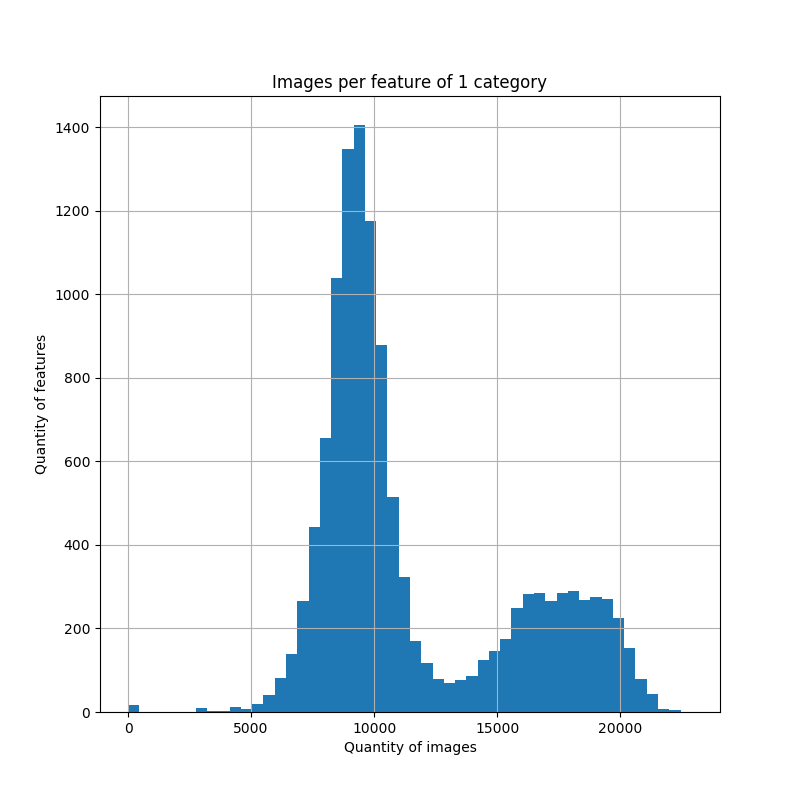
\includegraphics[width=\textwidth]  {Images/plots/25/Images_per_feature_of_1_category.png}
		\caption{Categoría 1}
	\end{subfigure}       
	\caption{Imágenes por categoría \label{fig:imagesperfeature}}
\end{figure}

En la figura \ref{fig:imagesperfeature} tenemos la distribución de las imágenes por categoría, es decir cuantas imágenes tienen una cierta cantidad de \textit{features}. En las tres categorías se ven dos distribuciones bien diferenciadas, lo que hace plantearse si depende de los dos tipos de capas diferentes del \textit{embedding} (las convolucionales y las completas).

\subsubsection{Synsets}

Como comentamos en la sección anterior los \textit{synsets} que hemos tomado son \ref{fig:synsets}. 
El criterio que hemos utilizado para decidir que una categoría pertenece a un \textit{synset} es que sea hipónimo de esta, por tanto es coherente que los \textit{synsets} más generales tengan más imágenes. 
 
Además, ambas familias(la de seres vivos y objetos), se distribuyen de forma parecida(cada \textit{synset} hijo tiene aproximadamente la mitad de imágenes que su \textit{synset} padre), como podemos ver en la figura \ref{fig:totalsynsets}. Elegimos dos familias de \textit{synsets} que cumplieran esto para que al comparar los resultados se distorsionaran lo menos posible por la cantidad de imágenes pertenecientes a ellas.

\begin{figure}[H] 
	\centering
	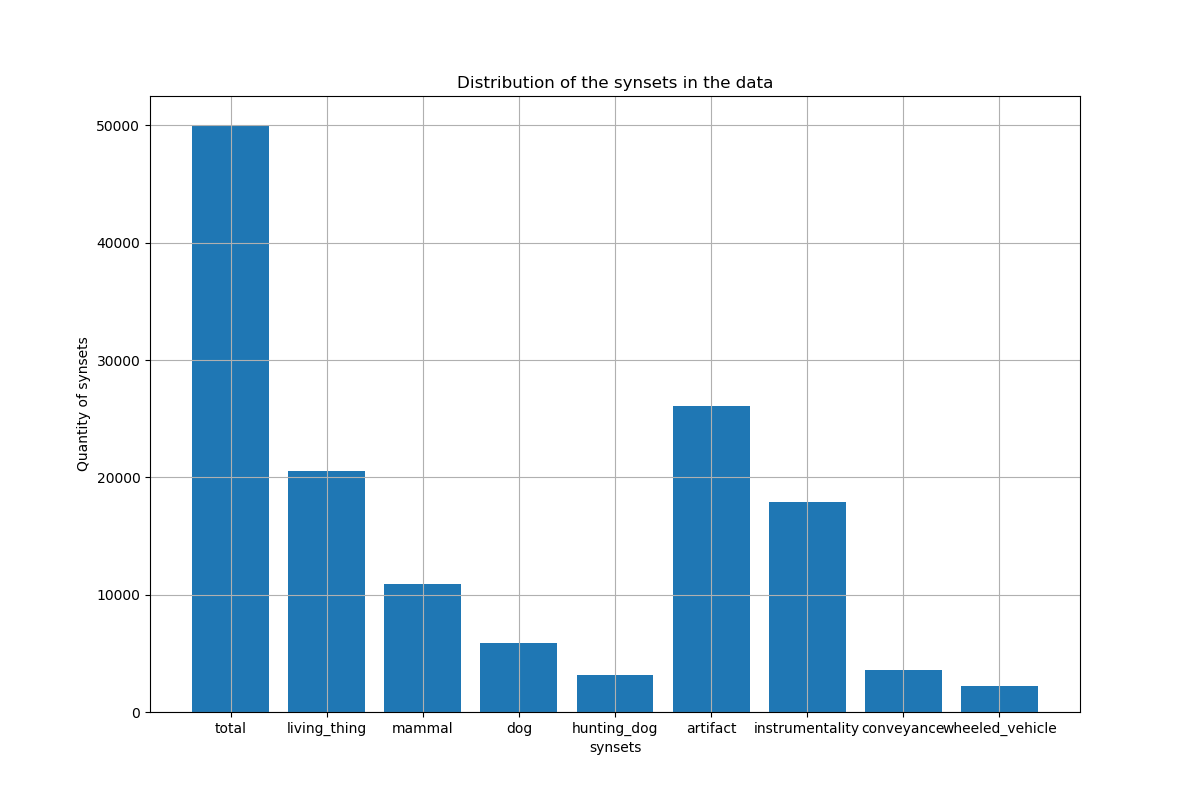
\includegraphics[width=0.8\textwidth] {Images/plots/25/distribution_of_synsets_bar.png}
	\caption{ 
	\label{fig:totalsynsets}}
\end{figure}


\subsection{Hipótesis iniciales}
Por la naturaleza del problema y lo que hemos visto al estudiar la matriz de embedding aparecen las siguientes hipótesis: 
\begin{itemize}
\item Las características se distribuyen de diferente manera en los layers convolucionales y los completos.

\item Cuanto más concreto es un synset, debería haber más features representativas, tanto por ausencia como por presencia.
\item Cuanto más profundo es el layer, debería haber más features representativas, tanto por ausencia como por presencia.
\item Se puede ver una relación entre los embeddings de synsets hipónimos.
\end{itemize}



\newpage
\section{Análisis}
\subsection{De wordnet a full network embedding}
En este apartado explicaré: 

\begin{itemize}
\item Las distribuciones de las imágenes por feature son diferentes para conv y fc, y mantienen la forma entre embeddings.
\item Las distribuciones de las imágenes por feature por layer por synset se conservan. 
\item Explicar los resultados de las matrices de cambio. 
\item Cuanto más concreto es el synset mayor proprción de 1. 

\end{itemize}



\subsection{Del full network embedding a wordnet}

Explicación de la distancia definida entre los synsets, demostración de que es distancia, los grafos con las distancias. 



%La idea principal de tfg es buscar relaciones entre los synsets de wordnet y el full network embedding. 
%Hipótesis iniciales: 
%- cuanto más concreto sea el synset más 1 debería tener.
%- Cuanto más profundo sea el layer más 1.


\section{Estructura del TFG: }

\begin{itemize}
\item \textbf{Introducción (5 pags): }
\begin{itemize}
\item FNN (Explicar neural networks, me puedo inspirar en \url{https://upc-mai-dl.github.io/mlp-convnets-theory/})
\item CNN 
\item EMbeddings  (Transfer Learning)
\end{itemize}
\item \textbf{Related Work (10 pags):}
\begin{itemize}
\item FNE 
\item Wordnet 
\item imagenet 
\end{itemize}
\item \textbf{Approach }
\begin{itemize}
\item Hipotesis iniciales 
\item statistics 
\item insights 
\end{itemize}
\item \textbf{Analysis}
\begin{itemize}
\item De wordnet a fne: Dado el embedding hemos encontrado patrones con los distintos synsets que concuerdan con las hipótesis
\item De fne a wordnet: Dado el árbol sintáctico y los patrones anteriores podemos generar una distancia con la que representamos lo parecidos que son los siynsets para la imagen. 
\end{itemize}
\end{itemize}

%\section{Introducción}
\newpage

\begin{thebibliography}{9}
\bibitem{dario}
\url{https://upc-mai-dl.github.io/mlp-convnets-theory/}

\bibitem{stanford} 
\url{http://cs231n.stanford.edu/}. 

\bibitem{fne} 
Dario Garcia-Gasulla, Armand Vilalta, Ferran Parés, Jonatan Moreno, Eduard Ayguadé, Jesus Labarta, Ulises Cortés, Toyotaro Suzumura, 
\textit{An Out-of-the-box Full-network Embedding for
Convolutional Neural Networks}.En arXiv:1705.07706,2017, \url{https://arxiv.org/abs/1705.07706}. 


\bibitem{wikiconv}
\url{https://en.wikipedia.org/wiki/Convolutional_neural_network#Convolutional}

\bibitem{deeplearningbook}
Deep Learning
Ian Goodfellow
Yoshua Bengio
Aaron Courville


\bibitem{behaviourcnn}
Dario Garcia-Gasulla, Ferran Parés, Armand Vilalta, Jonatan Moreno, Eduard Ayguadé, Jesús
Labarta, Ulises Cortés, and Toyotaro Suzumura. On the behavior of convolutional nets for
feature extraction. arXiv preprint arXiv:1703.01127, 2017.


\bibitem{imagencnn}
\url{https://leonardoaraujosantos.gitbooks.io/artificial-inteligence/content/neural_networks.html}

\end{thebibliography}
%Bishop - Pattern Recognition And Machine Learning.pdf
%Introduction to machine learning Ethem Alpaydın
%http://cs231n.stanford.edu/
%https://upc-mai-dl.github.io/mlp-convnets-theory/#adaptative_methods
%Apuntes de aprendizaje automático de Belanche
%______________________________________________________________
\appendix
\vfill\newpage 
\section{Glosario}
\begin{itemize}
\item Fordward pass: 
\item Sobreajuste: 
\item Kernel
\item Deep Network:
\item Hiperparámetros
\item Valores de activación de una red neuronal
\end{itemize}



\section{Código utilizado}
\begin{minted}{python}
class Data:
    """
    Esta clase consiste en los datos que voy a necesitar para hacer las estadísticas.
    Que no dependen de los synsets elegidos.

    Attributes:
        version (int): versión del embedding que utilizo puede ser 19, 25 o 31
        embedding_path (str): path
        layers (dict): Un diccionario tal que
            layers[string correspondiente al layer] = [inicio del layer, final del layer]

         labels ()

         :parameter version = Version del embedding que utilizo
    """

    def __init__(self, path, version=25):
        """

        :param version: Es la versión del embedding que queremos cargar (25,31,19)
        """
        self.version = version
        _embedding_path = "../Data/vgg16_ImageNet_ALLlayers_C1avg_imagenet_train.npz"
        self.imagenet_id_path = "../Data/synset.txt"
        if version == 25:
            _embedding = 'vgg16_ImageNet_imagenet_C1avg_E_FN_KSBsp0.15n0.25_Gall_train_.npy'
        elif version == 19:
            _embedding = 'vgg16_ImageNet_imagenet_C1avg_E_FN_KSBsp0.11n0.19_Gall_train_.npy'
        elif version == 31:
            _embedding = 'vgg16_ImageNet_imagenet_C1avg_E_FN_KSBsp0.19n0.31_Gall_train_.npy'
        else:
            _embedding = path
            print('No has puesto un embedding válido, usando el de defoult (25)')
        self.discretized_embedding_path = '../Data/Embeddings/' + _embedding
        print('Estamos usando ' + _embedding[-20:-16])
        embedding = np.load(_embedding_path)
        self.labels = embedding['labels']
        # self.matrix = self.embedding['data_matrix']
        del embedding
        self.dmatrix = np.array(np.load(self.discretized_embedding_path))
        self.imagenet_all_ids = np.genfromtxt(self.imagenet_id_path, dtype=np.str)
        self.features_category = [-1, 0, 1]
        self.colors = ['#3643D2', 'c', '#722672', '#BF3FBF']
        self.layers = {
            'conv1_1': [0, 64],  # 1
            'conv1_2': [64, 128],  # 2
            'conv2_1': [128, 256],  # 3
            'conv2_2': [256, 384],  # 4
            'conv3_1': [384, 640],  # 5
            'conv3_2': [640, 896],  # 6
            'conv3_3': [896, 1152],  # 7
            'conv4_1': [1152, 1664],  # 8
            'conv4_2': [1664, 2176],  # 9
            'conv4_3': [2176, 2688],  # 10
            'conv5_1': [2688, 3200],  # 11
            'conv5_2': [3200, 3712],  # 12
            'conv5_3': [3712, 4224],  # 13
            'fc6': [4224, 8320],  # 14
            'fc7': [8320, 12416],  # 15
            'conv1': [0, 128],  # 16
            'conv2': [128, 384],  # 17
            'conv3': [384, 1152],  # 18
            'conv4': [1152, 2688],  # 19
            'conv5': [2688, 4224],  # 20
            'conv': [0, 4224],  # 21
            'fc6tofc7': [4224, 12416],  # 23
            # 'all':[0,12416]          # 24
        }
        self.reduced_layers = {
            'conv1': [0, 128],
            'conv2': [128, 384],
            'conv3': [384, 1152],
            'conv4': [1152, 2688],
            'conv5': [2688, 4224],
            'fc6': [4224, 8320],
            'fc7': [8320, 12416]
        }

    def __del__(self):
        self.embedding = None
        self.dmatrix = None
        self.version = None
        self.embedding_path = None
        self.layers = None
        self.labels = None
        self.features_category = None
        self.colors = None
        gc.collect()


\end{minted}


\end{document}


